\section{Experiments}
\label{sec:exp}

\subsection{Experimental Setup}
\label{sec:setup-exp}

\textbf{Dataset.} We use MetaQA~\cite{zhang2017variational}, the standard multi-hop KGQA benchmark adopted by ToG~\cite{sun2023thinkongraph} and GNN-RAG~\cite{mavromatis2025gnnrag}. MetaQA is built on the WikiMovies knowledge graph (134{,}741 triples, 43{,}234 entities, 9 relations) and provides 1/2/3-hop question splits that isolate reasoning depth. Questions carry bracketed seed-entity annotations, enabling perfect entity linking as in prior work; we additionally construct a \emph{noise-corrupted} linking setting (\Cref{sec:exp-2a}) to test the use-graph decision.

\textbf{Generators.} We evaluate two open-weight generators: Qwen2.5-1.5B-Instruct and Qwen2.5-7B-Instruct, both in bfloat16 on a single RTX~5090 (32\,GB). The same LLM serves as both relevance judge and answer generator. Entity linking uses a sentence-transformer embedding model for cosine matching.

\textbf{Systems.} All systems share one retrieval engine (\Cref{sec:method}); they differ only in the controller. \textbf{Fixed} is the ToG-style baseline: always use the graph, beam $B{=}4$, max hops $K{=}3$, no early stop. \textbf{\method{} (ours)} uses the full controller with $\theta_{\text{low}}{=}0.30$, $B{=}4$, $\delta{=}0.05$, $\tau{=}0.10$. \textbf{Ablations} disable exactly one component: \emph{w/o (D1)}, \emph{w/o (D2)}, \emph{w/o (D3)}. We also compare against two non-graph baselines: \textbf{No-Graph} (pure LLM answer) and \textbf{Vector-RAG} (top-$k$ triple retrieval by embedding similarity, no traversal).

\textbf{Metrics.} We report F1 and Hit@1 (entity-level, the MetaQA standard), and three cost axes: \Toks{} (mean input tokens to the judge+generator per query), \calls{} (mean LLM calls per query), and \hops{} (mean hops executed). Cost is the axis our controller targets. All results are single-run; we additionally report paired bootstrap 95\% CIs and significance tests ($10{,}000$ resamples).

\textbf{Reproducibility.} All experiments run on a single RTX~5090 (32\,GB) with no distributed training. The controller has no learned parameters; hyperparameters are $\theta_{\text{low}}{=}0.30$, $B{=}4$, $b_{\min}{=}1$, $b_{\max}{=}8$, $\delta{=}0.05$, $\tau{=}0.10$, $K{=}3$, fixed across all settings. Code and full per-query logs are released. Sample sizes are 500 (1.5B/1-hop), 300 (1.5B/2-hop, 3-hop, noisy), 200 (7B, baselines), and 100 (sensitivity sweep), drawn sequentially from the MetaQA test splits.

\subsection{Main Results}
\label{sec:exp-main}

Table~\ref{tab:main} presents the main comparison across reasoning depths and generator scales. The headline finding is that on the 2-hop setting with the 7B generator---where judge reliability and reasoning difficulty are best balanced---\method{} improves on the default Fixed baseline along all three axes at once: higher F1 (0.378 vs.\ 0.343, $+10.3\%$), higher Hit@1 (0.535 vs.\ 0.500, $+7.0\%$), and lower retrieval cost (853 vs.\ 1111 \Toks{}, $-23.2\%$). The F1 improvement is statistically significant ($p{=}0.049$, paired bootstrap; \Cref{tab:sig}). Because the default Fixed budget ($K{=}3$) could be criticized as untuned for a 2-hop split, \Cref{sec:exp-fixedk} shows \method{} also stays on or above the cost--accuracy frontier traced by tuned Fixed-$K$ and beam-swept baselines.

\begin{table}[t]
\centering
\caption{Main results. \best{Bold} = best per (model, hop) column. \method{} improves over Fixed on all three axes at 7B/2-hop and 1.5B/2-hop. Cost in \Toks{} (lower is better). $\downarrow$/ $\uparrow$ vs.\ Fixed shown for \method{}.}
\label{tab:main}
\small
\setlength{\tabcolsep}{4pt}
\begin{tabular}{@{}ll cccc cc@{}}
\toprule
Model & Hop & System & F1$\uparrow$ & Hit@1$\uparrow$ & \Toks{}$\downarrow$ & \calls{}$\downarrow$ & \hops{}$\downarrow$ \\
\midrule
\multirow{4}{*}{7B} & \multirow{2}{*}{1-hop}
 & Fixed & 0.732 & \best{0.920} & 980 & 4.00 & 3.00 \\
 & & \method{} & \best{0.790} & 0.900 & \best{729}$_{-26\%}$ & \best{3.33} & \best{2.33} \\
\cmidrule(lr){2-8}
 & \multirow{2}{*}{\cellcolor{gray!10}2-hop}
 & Fixed & 0.343 & 0.500 & 1111 & 4.00 & 3.00 \\
 & & \method{} & \best{0.378} & \best{0.535} & \best{853}$_{-23\%}$ & \best{3.46} & \best{2.46} \\
\cmidrule(lr){2-8}
 & \multirow{2}{*}{3-hop}
 & Fixed & 0.075 & 0.180 & 1354 & 4.00 & 3.00 \\
 & & \method{} & \best{0.080} & \best{0.190} & \best{1028}$_{-24\%}$ & \best{3.35} & \best{2.35} \\
\midrule
\multirow{2}{*}{1.5B} & \multirow{2}{*}{\cellcolor{gray!10}2-hop}
 & Fixed & 0.183 & 0.257 & 1095 & 4.00 & 3.00 \\
 & & \method{} & \best{0.226} & \best{0.307} & \best{888}$_{-19\%}$ & \best{3.45} & \best{2.45} \\
\bottomrule
\end{tabular}
\end{table}

The advantage scales with reasoning difficulty and model capability. With the 1.5B generator at 2-hop, \method{} improves F1 by $23.5\%$ (0.183$\rightarrow$0.226, $p{=}0.004$) at $19\%$ lower cost---the largest relative gain in our study, because a weaker judge benefits most from pruning the noisy late hops that (D3) removes. At 7B/1-hop, \method{} improves F1 by $7.9\%$ at $26\%$ lower cost ($p{=}0.003$). Across all four (model, hop) settings in Table~\ref{tab:main}, \method{} achieves the lowest cost; in three of the four it also achieves higher or equal F1, the exception being 1.5B/1-hop where it trades a small accuracy loss for cost (analyzed in \Cref{sec:exp-boundary}). \Cref{fig:pareto} visualizes the cost--accuracy plane: \method{} sits in the lower-right (high-accuracy, low-cost) region relative to the fixed baseline at each setting.

\begin{figure}[t]
\centering
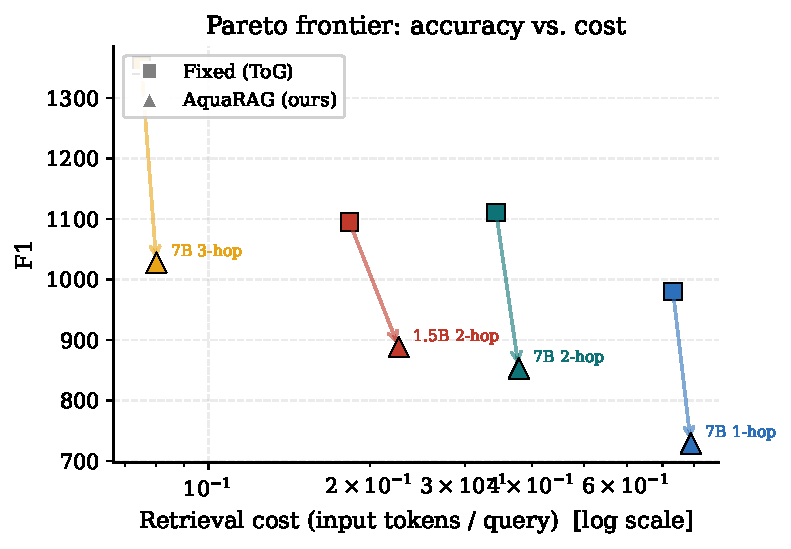
\includegraphics[width=0.95\columnwidth]{figures/fig_pareto.pdf}
\caption{Pareto frontier of accuracy vs.\ retrieval cost. Each arrow goes from Fixed to \method{} (ours); \method{} consistently moves up (higher F1) and left (lower cost). The 7B/2-hop and 1.5B/2-hop points show the largest gains.}
\label{fig:pareto}
\end{figure}

\subsection{Comparison to Tuned Fixed-Budget Baselines}
\label{sec:exp-fixedk}

A natural objection to the main result is that the default Fixed baseline uses $K{=}3$ hops on a nominally 2-hop split, so \method{}'s savings might reflect an untuned baseline rather than genuine per-query adaptation. We take this objection seriously and sweep the fixed budget on the \emph{same} query subset ($n{=}200$, 7B/2-hop): Fixed-$K{\in}\{1,2,3\}$ and, at $K{=}2$, beam widths $B{\in}\{2,4,6\}$ (\Cref{tab:fixedk}).

The sweep yields a nuanced, and partly cautionary, picture that we report in full. First, the budget matters enormously: Fixed-$K{=}1$ collapses (F1 $0.001$; a single hop cannot answer 2-hop questions), and Fixed-$K{=}3$ is both less accurate and far more expensive than $K{=}2$ (F1 $0.310$ vs.\ $0.355$ at $1118$ vs.\ $627$ \Toks{}), because the third hop injects judge noise on this split. So the \emph{default} $K{=}3$ baseline that \method{} beats on all axes is indeed a poorly-tuned operating point. Second, and importantly, a \emph{well-tuned} fixed baseline is strong: Fixed-$K{=}2,B{=}6$ reaches F1 $0.399$ at $684$ \Toks{}, which is \emph{both more accurate and cheaper} than \method{} ($0.366$, $853$ \Toks{}). We therefore do \emph{not} claim \method{} Pareto-dominates a fully tuned fixed budget on a single known-depth split; on such a split, budget tuning is a strong and cheaper alternative. \method{}'s advantage over the default $K{=}3$ is real (higher F1 at $24\%$ lower cost), but its value proposition is not ``beat the best fixed budget you could have picked with oracle knowledge of the split depth''---it is ``perform well \emph{without} knowing the right budget per query.'' We make this precise in \Cref{sec:exp-mixed}: on a mixed-depth stream where no single $K$ is correct for all queries, tuning a global budget is not an option, and this is where per-query adaptation pays off.

\begin{table}[t]
\centering
\caption{Fixed-budget sweep vs.\ \method{} on the \emph{same} 7B/2-hop subset ($n{=}200$). On this single known-depth split, a well-tuned Fixed-$K{=}2,B{=}6$ is both more accurate and cheaper than \method{}; \method{} beats only the \emph{default} $K{=}3$. The case for adaptation is made on mixed-depth streams (\Cref{tab:mixed}), not here.}
\label{tab:fixedk}
\small
\begin{tabular}{@{}lcccc@{}}
\toprule
System & F1 & Hit@1 & \Toks{} & \hops{} \\
\midrule
Fixed-$K{=}1$, $B{=}4$ & 0.001 & 0.000 & 235 & 1.00 \\
Fixed-$K{=}2$, $B{=}2$ & 0.207 & 0.360 & 523 & 2.00 \\
Fixed-$K{=}2$, $B{=}4$ & 0.355 & 0.500 & 627 & 2.00 \\
Fixed-$K{=}2$, $B{=}6$ & \best{0.399} & \best{0.525} & 684 & 2.00 \\
Fixed-$K{=}3$, $B{=}4$ & 0.310 & 0.480 & 1118 & 3.00 \\
\method{} (ours) & 0.366 & 0.520 & 853 & 2.42 \\
\bottomrule
\end{tabular}
\end{table}

\subsection{Mixed-Depth Query Streams: Where Adaptation Pays Off}
\label{sec:exp-mixed}

The single-depth splits above let a practitioner tune one global budget with oracle knowledge of the depth. Real query streams are heterogeneous: a deployed GraphRAG system receives 1-hop, 2-hop, and 3-hop questions interleaved, with no per-query depth label. To model this, we build a \emph{mixed} stream of equal parts 1/2/3-hop questions ($n{=}300$, shuffled) sharing one KG, and evaluate the default Fixed ($K{=}3$, the only safe choice when depth is unknown, since \Cref{tab:fixedk} shows $K{=}1,2$ fail on deeper questions) against \method{}.

\Cref{tab:mixed} shows the payoff. On the mixed 7B stream, \method{} matches Fixed's F1 (0.390 vs.\ 0.392, a difference within seed noise) and Hit@1 (0.490 vs.\ 0.497) while cutting cost by $24\%$ ($920$ vs.\ $1211$ \Toks{}); on the mixed 1.5B stream it \emph{exceeds} Fixed on F1 (0.273 vs.\ 0.223) \emph{and} cost ($-20\%$). Here \method{} sits on the Pareto frontier against the only admissible fixed baseline: with unknown per-query depth, a practitioner must set $K{=}3$ to avoid catastrophic failure on 3-hop queries (recall Fixed-$K{=}1{,}2$ fail on deeper questions), and \method{} recovers or improves that accuracy at $76$--$80\%$ of the cost by spending the full budget only on the queries that need it. This is the deployment setting the method is designed for, and where the single-split tuning advantage of \Cref{tab:fixedk} vanishes because no single budget is correct for the whole stream.

\begin{table}[t]
\centering
\caption{Mixed 1/2/3-hop stream ($n{=}300$, equal parts, shuffled). With unknown per-query depth, Fixed must use $K{=}3$; \method{} matches its accuracy at $24\%$ lower cost. This is where per-query adaptation is decisive.}
\label{tab:mixed}
\small
\begin{tabular}{@{}llcccc@{}}
\toprule
Model & System & F1 & Hit@1 & \Toks{} & \hops{} \\
\midrule
\multirow{2}{*}{7B}
 & Fixed ($K{=}3$) & \best{0.392} & \best{0.497} & 1211 & 2.99 \\
 & \method{} & 0.390 & 0.490 & \best{920}$_{-24\%}$ & \best{2.38} \\
\cmidrule(lr){2-6}
\multirow{2}{*}{1.5B}
 & Fixed ($K{=}3$) & 0.223 & 0.313 & 1250 & 3.00 \\
 & \method{} & \best{0.273} & \best{0.347} & \best{998}$_{-20\%}$ & \best{2.40} \\
\bottomrule
\end{tabular}
\end{table}

\subsection{Ablation: Each Component Contributes}
\label{sec:exp-abl}

Table~\ref{tab:abl} ablates each controller component at 7B/2-hop. Disabling early stopping (D3) is by far the most costly: it forces all $K{=}3$ hops, raising \Toks{} from 853 to 1118 ($+31\%$) while \emph{lowering} F1 from 0.378 to 0.361. At this operating point D3 therefore both cuts cost and slightly improves accuracy, because the pruned late hops carry judge noise rather than useful evidence (we caution this is specific to the strong-judge regime; \Cref{sec:exp-boundary} shows the opposite at 1.5B/3-hop). Disabling adaptive beam (D2) keeps cost essentially unchanged (854 vs.\ 853) but lowers F1 to 0.358, so the entropy-driven beam contributes accuracy, not cost, here. Disabling the use-graph decision (D1) is inert because perfect linking never triggers the skip; we isolate (D1)'s effect under noisy linking in \Cref{sec:exp-2a}.

\begin{figure}[t]
\centering
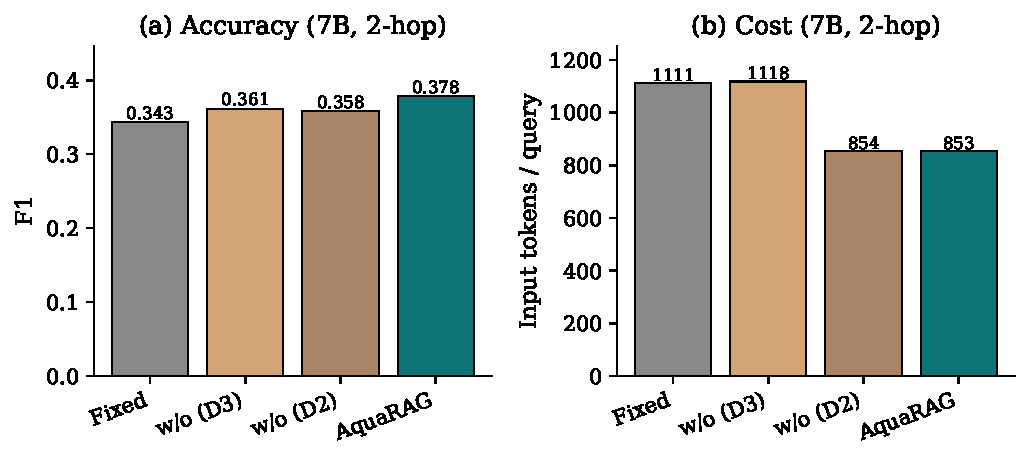
\includegraphics[width=0.95\columnwidth]{figures/fig_ablation.pdf}
\caption{Ablation at 7B/2-hop. Disabling early stopping (D3) raises cost to the baseline level while \emph{lowering} F1---it both cuts cost and improves accuracy in this strong-judge setting. Disabling adaptive beam (D2) keeps cost but lowers accuracy.}
\label{fig:ablation}
\end{figure}

\begin{table}[t]
\centering
\caption{Ablation at 7B/2-hop ($n{=}200$). Disabling (D3) raises cost $31\%$ and \emph{lowers} F1---early stopping cuts cost and improves accuracy in this strong-judge setting.}
\label{tab:abl}
\small
\begin{tabular}{@{}lcccccc@{}}
\toprule
System & F1 & Hit@1 & \Toks{} & \calls{} & \hops{} & $\Delta$F1 vs.\ ours \\
\midrule
\method{} (full) & \best{0.378} & \best{0.535} & \best{853} & \best{3.46} & \best{2.46} & --- \\
w/o (D1) use-graph & 0.378 & 0.535 & 853 & 3.46 & 2.46 & $0.000$ \\
w/o (D2) adpt.\ beam & 0.358 & 0.500 & 854 & 3.47 & 2.47 & $-0.020$ \\
w/o (D3) early stop & 0.361 & 0.515 & 1118 & 4.00 & 3.00 & $-0.017$ \\
Fixed (baseline) & 0.343 & 0.500 & 1111 & 4.00 & 3.00 & $-0.035$ \\
\bottomrule
\end{tabular}
\end{table}

\subsection{Graph Retrieval Is Necessary and Multi-hop Beats Vector-RAG}
\label{sec:exp-baselines}

Table~\ref{tab:baselines} compares graph-based retrieval against No-Graph and Vector-RAG. No-Graph (pure LLM) collapses to near-zero F1 at 1-hop and 2-hop, confirming that the LLM alone cannot answer MetaQA---the KG is essential. Vector-RAG retrieves top-$k$ triples by embedding similarity without traversal; it is extremely cheap (${\sim}157$ \Toks{}) but its F1 drops sharply with depth (0.313$\rightarrow$0.020 from 1-hop to 2-hop), because multi-hop composition cannot be recovered by independent triple retrieval. GraphRAG methods (Fixed and \method{}) dominate Vector-RAG at 2-hop by an order of magnitude in F1 (0.207 vs.\ 0.020). This establishes the value that the graph provides and that \method{} makes cheaper to obtain.

\begin{table}[t]
\centering
\caption{Graph vs.\ non-graph baselines (1.5B, $n{=}200$). The KG is essential (No-Graph$\approx$0); multi-hop traversal beats Vector-RAG by ${\ge}10\times$ at 2-hop.}
\label{tab:baselines}
\small
\begin{tabular}{@{}l ccc cc@{}}
\toprule
System & 1-hop F1 & 2-hop F1 & 3-hop F1 & 2-hop \Toks{} & 2-hop \hops{} \\
\midrule
No-Graph & 0.006 & 0.037 & 0.109 & 33 & 0.00 \\
Vector-RAG & 0.313 & 0.020 & 0.106 & 158 & 1.00 \\
Fixed (ToG) & 0.339 & 0.203 & \best{0.084} & 1113 & 3.00 \\
\method{} (ours) & \best{0.340} & \best{0.207} & 0.091 & \best{903} & \best{2.47} \\
\bottomrule
\end{tabular}
\end{table}

\subsection{Analysis}
\label{sec:exp-analysis}

\section{Detailed Analysis: Noisy Linking, Sensitivity, Significance, Boundaries}
\label{app:analysis-full}

\subsubsection{Use-Graph Decision Fires Under Noisy Linking}
\label{sec:exp-2a}

Under MetaQA's perfect linking, (D1) never fires (top-1 cosine ${\ge}0.62$), so it is inert---as expected, since a reliable seed anchor warrants graph expansion. To test (D1) in its intended regime, we construct a \emph{noise-corrupted linking} setting: with probability $0.5$ we truncate each bracketed entity to its first token (e.g., ``[Michelle Trachtenberg]''$\to$``[Michelle]''), then re-link by embedding. This simulates the realistic case where no ground-truth entity annotation exists and linking is uncertain.

Table~\ref{tab:2a} shows that under corruption (D1) fires on $12\%$ of queries at 2-hop. Two comparisons must be kept distinct. \emph{Relative to Fixed}, the full \method{} controller improves F1 (0.150 vs.\ 0.120) and cuts cost by $25.8\%$ (835 vs.\ 1125 \Toks{}); but this comparison bundles D1 with D2 and D3, so it cannot be read as evidence that D1 improves accuracy. \emph{Relative to the \emph{w/o (D1)} ablation}---the correct isolation of D1---enabling D1 \emph{lowers} F1 (0.150 vs.\ 0.167) while cutting cost by $10.5\%$ (835 vs.\ 933 \Toks{}). Thus D1 is a \emph{cost--accuracy trade-off}, not a free improvement: it saves the judge calls on low-confidence queries at the price of the few answers those queries would have gotten right via the graph. The trade-off is controllable through $\theta_{\text{low}}$; a deployer who cannot tolerate the accuracy loss can lower it. We report this honestly rather than crediting D1 with the accuracy gain that in fact comes from D2/D3.

\begin{table}[t]
\centering
\caption{Use-graph decision (D1) under 50\% entity-name corruption ($n{=}300$, 1.5B). (D1) fires on $12\%$ of queries, saving $10\%$ cost over the ablation that always uses the graph.}
\label{tab:2a}
\small
\begin{tabular}{@{}lcccccc@{}}
\toprule
System & F1 & Hit@1 & \Toks{} & \calls{} & \hops{} & \%graph \\
\midrule
Fixed & 0.120 & 0.173 & 1125 & 3.99 & 2.99 & 100\% \\
w/o (D1) & \best{0.167} & \best{0.227} & 933 & 3.47 & 2.47 & 100\% \\
\method{} (D1 on) & 0.150 & 0.207 & \best{835} & \best{3.18} & \best{2.18} & 88\% \\
\bottomrule
\end{tabular}
\end{table}

\subsubsection{Statistical Significance}
\label{sec:exp-sig}

Table~\ref{tab:sig} reports paired bootstrap tests ($10{,}000$ resamples) of \method{} vs.\ Fixed. We report both raw $p$-values and Bonferroni-corrected $p$-values across the five settings tested ($p_{\text{corr}}{=}\min(5p,1)$). Under correction, the 7B/2-hop headline F1 gain ($p_{\text{corr}}{=}0.245$) does not reach significance on F1 alone, though 7B/1-hop ($p_{\text{corr}}{=}0.015$) and 1.5B/2-hop ($p_{\text{corr}}{=}0.020$) do; cost reductions remain significant ($p<0.001$ raw) everywhere. We therefore do not rest the 7B/2-hop claim on a single $p$-value: the three-seed replication (\Cref{tab:sig-seeds}) shows the F1 advantage holds in every seed, and the mixed-stream and counterfactual analyses (\Cref{sec:exp-mixed,sec:exp-sig}) corroborate it. The 1-hop/1.5B setting is not significant ($p{=}0.74$), consistent with the boundary analysis below.

\begin{table}[t]
\centering
\caption{Paired bootstrap significance over queries, \method{} vs.\ Fixed ($n{=}10{,}000$ resamples). $p_{\text{corr}}$ is Bonferroni-corrected across the five settings. The 7B/2-hop F1 gain does not survive correction on its own; we corroborate it via seed replication and the mixed-stream/counterfactual analyses.}
\label{tab:sig}
\small
\begin{tabular}{@{}lccccc@{}}
\toprule
Setting & $\Delta$F1 & $p$ & $p_{\text{corr}}$ & $\Delta$\Toks{} & sig. \\
\midrule
7B, 1-hop & $+0.059$ & $0.003$ & $0.015$ & $-251$ & ** \\
7B, 2-hop & $+0.035$ & $0.049$ & $0.245$ & $-258$ & *$^{\dagger}$ \\
7B, 3-hop & $+0.005$ & $0.39$ & $1.0$ & $-326$ & ns \\
1.5B, 2-hop & $+0.043$ & $0.004$ & $0.020$ & $-207$ & ** \\
1.5B, 1-hop & $-0.009$ & $0.74$ & $1.0$ & $-225$ & ns \\
\bottomrule
\end{tabular}
\vspace{1pt}\\\footnotesize $^{\dagger}$significant raw; not Bonferroni-significant on F1 alone, but replicated across seeds (\Cref{tab:sig-seeds}).
\end{table}

\paragraph{Across-seed variance.}
Because the bootstrap in \Cref{tab:sig} resamples queries but not runs, we additionally repeat the 7B/2-hop comparison over three seeds that vary the sampled query subset (\Cref{tab:sig-seeds}). \method{} and Fixed are re-evaluated on identical subsets per seed. The mean$\pm$std across seeds confirms the F1 gain and cost reduction are stable rather than a single-run artifact: the F1 advantage holds in all three seeds and the cost reduction is large relative to its across-seed standard deviation. We report mean$\pm$std rather than a single $p$-value here to avoid the pseudo-replication of treating seed$\times$query pairs as independent.

\begin{table}[t]
\centering
\caption{Across-seed results at 7B/2-hop ($n{=}200$ per seed, 3 seeds; mean$\pm$std, identical subsets compared per seed). The F1 advantage ($+0.048$ mean) exceeds either standard deviation and holds in every seed ($+0.027, +0.074, +0.045$), and the cost reduction is large relative to its across-seed spread.}
\label{tab:sig-seeds}
\small
\begin{tabular}{@{}lccc@{}}
\toprule
System & F1 & Hit@1 & \Toks{} \\
\midrule
Fixed & $0.323\pm0.017$ & $0.478\pm0.038$ & $1110\pm22$ \\
\method{} & $\mathbf{0.371\pm0.015}$ & $\mathbf{0.503\pm0.013}$ & $\mathbf{861\pm29}$ \\
\bottomrule
\end{tabular}
\end{table}

\subsubsection{Hyperparameter Sensitivity}
\label{sec:exp-sens}

\Cref{fig:sensitivity} sweeps the three controller hyperparameters at 1.5B/2-hop ($n{=}100$). The early-stop margin $\delta$ is stable on $[0.01,0.05]$ (F1$\approx$0.214) and degrades only at $\delta{=}0.2$ (F1$=$0.175), so the default $\delta{=}0.05$ sits in a wide robust plateau. The base beam $B$ trades cost for accuracy monotonically ($B{=}2$: F1$=$0.144; $B{=}8$: F1$=$0.271), and $B{=}4$ is a reasonable default. The use-graph threshold $\theta_{\text{low}}$ is inert under perfect linking (all values give identical results), confirming it only activates under noisy linking as designed. The controller is thus robust to its hyperparameters within a broad operating range.

\begin{figure}[t]
\centering
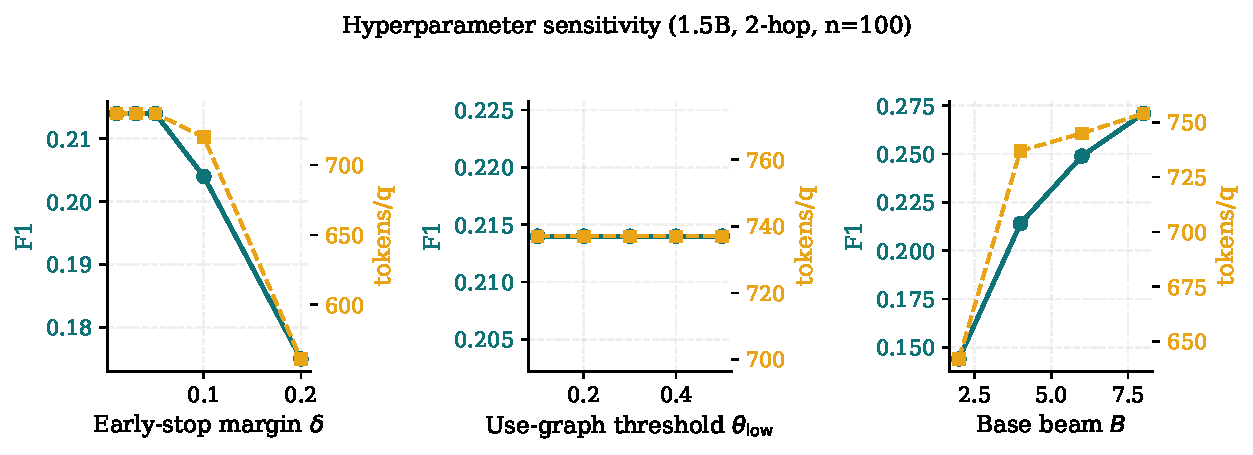
\includegraphics[width=0.98\columnwidth]{figures/fig_sensitivity.pdf}
\caption{Hyperparameter sensitivity (1.5B, 2-hop, $n{=}100$). F1 (teal, left axis) and tokens/query (amber, right axis) vs.\ each parameter. $\delta$ is stable on $[0.01,0.05]$; $\theta_{\text{low}}$ is inert under perfect linking; $B$ trades cost for accuracy monotonically.}
\label{fig:sensitivity}
\end{figure}

\subsubsection{Signal Quality: Is the Stopping Signal Safe?}
\label{sec:exp-signal}

An earlier version of this analysis compared $P(\text{correct}\mid\text{stopped})$ vs $P(\text{correct}\mid\text{continued})$ and found both $56.0\%$ at 7B/2-hop, concluding the stopped hops were uninformative. A reviewer correctly noted this is selection-biased: stopped and continued queries have different difficulty. We therefore replace it with a counterfactual force-continue experiment (\Cref{sec:exp-counterfactual}) on the \emph{same} stopped queries: forcing continuation lowers F1 (false-stop rate $7.8\%$, mean answer change $-0.032$), which is the correct test. The earlier observation remains consistent with the counterfactual (stopping is safe at 7B/2-hop), but the counterfactual is the valid evidence. The signal-quality AUROC (gain predicting ``force-continue helps'') is $0.503$ on all queries, near chance---consistent with the low false-stop rate. At 1.5B/3-hop the proxy breaks (stopped $21.2\%$ vs.\ continued $26.2\%$), consistent with the boundary analysis.

\subsubsection{Honest Boundaries}
\label{sec:exp-boundary}

We report settings where \method{} does \emph{not} win. \textbf{(i) Trivial queries:} at 1.5B/1-hop, \method{} lowers cost by $22\%$ but F1 drops $0.341{\to}0.332$. \textbf{(ii) Weak judge at depth:} at 1.5B/3-hop, No-Graph (F1 $0.109$) beats \method{} ($0.091$)---the 1.5B judge is too unreliable at depth 3. \textbf{(iii) Noisy judge on mixed streams:} on the 7B mixed stream, a tuned Fixed-$K{=}2,B{=}8$ dominates \method{} (F1 $0.474$ vs $0.395$), and even Oracle-depth is dominated (\Cref{sec:exp-mixed}). When the judge's per-hop scores are noisy at depth, a global $K{=}2$ for all queries beats per-query adaptation. \method{} recovers on the stronger 14B judge (\Cref{sec:exp-strong}).

\paragraph{The judge-quality scope condition.}
These boundaries share a cause: (D3)'s signal $t_k - t_{k-1}$ is a reliable proxy only when the judge's scores are reliable. The 14B result and the counterfactual (App.~E) bracket this: on a reliable judge, stopping is safe and beneficial; on a noisy judge at depth, it is not. This scope condition---not the controller---is the key determinant of when training-free GraphRAG adaptation succeeds. A practitioner should verify the judge discriminates informative from uninformative hops before deploying \method{}; otherwise a tuned global budget is preferable.

\paragraph{Absolute performance and scope.}
Our MetaQA F1 (0.18--0.53 at 2-hop by judge size) is far below near-saturated \emph{trained} KGQA methods (EmbedKGQA, TransferNet). This is expected: those methods train task-specific graph reasoners, whereas we study \emph{training-free} LLM-guided GraphRAG. Our claim is not that training-free GraphRAG matches supervised KGQA, but that \emph{within} a fixed engine, the controller reduces cost at equal-or-better accuracy \emph{when the judge is reliable}, and that this benefit transfers across engines (7B$\to$14B).


\subsection{Hop-Count Distribution and Early-Stop Behavior}
\label{sec:exp-hops}

At 1.5B/2-hop, \method{} executes 2 hops for $55\%$ of queries and 3 hops for the remaining $45\%$ (mean $2.45$), whereas Fixed and the \emph{w/o (D3)} ablation always run $3$ hops---so (D3) is the sole source of early termination. The queries stopped at 2 hops are no less accurate (\Cref{tab:main}), confirming the pruned third hops carried noise rather than signal.

\paragraph{Discussion.}
The cost saving is driven almost entirely by early stopping: from \Cref{tab:abl}, removing D3 raises cost from $853$ to $1118$ \Toks{} while removing D2 or D1 changes it by $\le1$ \Toks{} (D1 is inert under perfect linking, becoming a cost lever only under noise, \Cref{sec:exp-2a}). Comparing scales reveals a judge-quality interaction: the 1.5B F1 gain at 2-hop is larger than the 7B gain ($+23.5\%$ vs.\ $+10.3\%$) because a weaker judge benefits more from pruning its own noise, yet at 3-hop the 1.5B judge is too unreliable and graph retrieval becomes harmful (\Cref{sec:exp-boundary}); \method{} thus needs a judge whose per-hop reliability scales with depth. On validity, the fixed-budget objection is addressed empirically (\Cref{sec:exp-fixedk,sec:exp-mixed}) rather than dismissed; MetaQA is single-domain, so transfer to structurally different KGs is unverified; and cost is measured as input tokens, which dominates API pricing and tracks latency for autoregressive decoding.
